\documentclass[11pt,letter]{article}
\usepackage{amsmath, amsthm, amssymb}
\usepackage{eucal, mathrsfs, yfonts}
\usepackage{amsfonts}
\usepackage{amssymb}
\usepackage{amsmath}
\usepackage{amsthm}
\usepackage{verbatim}
\usepackage{fancyhdr}
\usepackage{geometry}
\usepackage{setspace}
\usepackage{Tabbing}
\usepackage{lastpage}
\usepackage{extramarks}
\usepackage{chngpage}
\usepackage{soul,color}
\usepackage{graphicx,float,wrapfig}
\usepackage[urlcolor=blue]{hyperref}
\hypersetup{colorlinks=true}

\graphicspath{{./Pictures/}}

%code preamble
\usepackage{color}
\usepackage{xcolor}
\usepackage{listings}

\usepackage{caption}
\DeclareCaptionFont{white}{\color{white}}
\DeclareCaptionFormat{listing}{\colorbox{gray}{\parbox{\textwidth}{#1#2#3}}}
\captionsetup[lstlisting]{format=listing,labelfont=white,textfont=white}

\lstset{language=C++,
               basicstyle=\ttfamily\small,
               keywordstyle=\color{blue}\ttfamily,
               otherkeywords={WIDTH},
               keywords=[2]{__shared__},
               keywordstyle=[2]\color{orange}\ttfamily,
               stringstyle=\color{green}\ttfamily,
               commentstyle=\color{red}\ttfamily,
               breaklines=true,
}
%end code preamble

\topmargin=-0.45in      %
\evensidemargin=0in     %
\oddsidemargin=0in      %
\textwidth=6.5in        %
\textheight=9.0in       %
\headsep=0.25in         %


\newcommand{\HRule}{\rule{\linewidth}{0.5mm}}

\pagestyle{fancy}



\lhead{Asssignment 1}
\chead{UCID: 22365174}
\rhead{Arturo Pacifico Griffini}

\title{Assignment 1 }
\author{Arturo Pacifico Griffini\\
	UCID: 22365174}
\date{}

\begin{document}
%\maketitle
%\input{./title.tex}

\pagebreak

\section{Measuring Execution Time}

Print sum (on), hardcoded (off)\\*
--With -O2 enabled it takes 107938 ticks.\\*
--Without -O2 enabled it takes 147217 ticks.\\*
Print sum (on), hardcoded (on)\\*
--With -O2 enabled it takes 78011 ticks.\\*
--Without -O2 enabled it takes 139840 ticks.\\*
Print sum (off), hardcoded (off)\\*
--With -O2 enabled it takes 8021 ticks.\\*
--Without -O2 enabled it takes 69745 ticks.\\*
Print sum (off), hardcoded (on)\\*
--With -O2 enabled it takes 1245 ticks.\\*
--Without -O2 enabled it takes 67005 ticks.\\[10pt]

\noindent\emph{Discrepancy in timing:}\\*
O2 is a compiler flag that tells the compiler to optimise your code for performance. Hence, without the -O2 flag the code runs slower and it takes more 'ticks' to execute. Hardcoding, your inputs takes off the overhead of processing your inputs from the command line. e.g we need to make the string "10000" into and integer before we can use it. Hence hardcoding improves performance. Printf, also takes time to execute and therefore the additional ticks when we print the sum.\\[10pt]

\noindent\emph{Best Configuration:}\\*
The best config if: print off; hardcoded on; -O2 flag off. With this configuration we exclude the overhead of input/output processing and test the performance of the bare algorithm, since we do not let the compiler do any magic on it.\\[10pt]

\noindent\emph{What is argv:}\\*
Argv is an array of character arrays (strings) of length argc where the strings at index 1, ..., n are the inputs in the command line and argv[0] is the name of the executable. argv[1] = "10000" in our case.\\[10pt]

\noindent\emph{What is atoi():}\\*
atoi() is a function in the standard library that takes a string as argument and returns the corresponding integer.

\section{Measuring Memory Latency}

\noindent\emph{How does the pointer chase benchmark measure memory latency:}\\*
By accessing memory addresses in random order within a certain memory bound, you are not exploiting spatial locality. In a way, it is like writing code with no memory optimisation and therefore it gives you a good memory benchmark.\\[10pt]

\noindent\emph{Size in bytes of an array of ints of size n:}\\*
Size in bytes is $n \cdot sizeof(int)$. On the hive machines $sizeof(int) = 4$ bytes.\\[10pt]

\noindent\emph{Cycles per step vs the size of the array}\\*
The following is a plot showing the relationship between the average number of cycles to execute a step (vertical axis) and the size in bytes of the array (horizontal axis). The size varies from 32KBytes to approximately 8MBytes, with a step that increases by powers of 2. i.e. $X = {x | x = 32000 + 2^n}$ where $n$ is an integer between 0 and 21 included.
\begin{figure}[h]
\centering
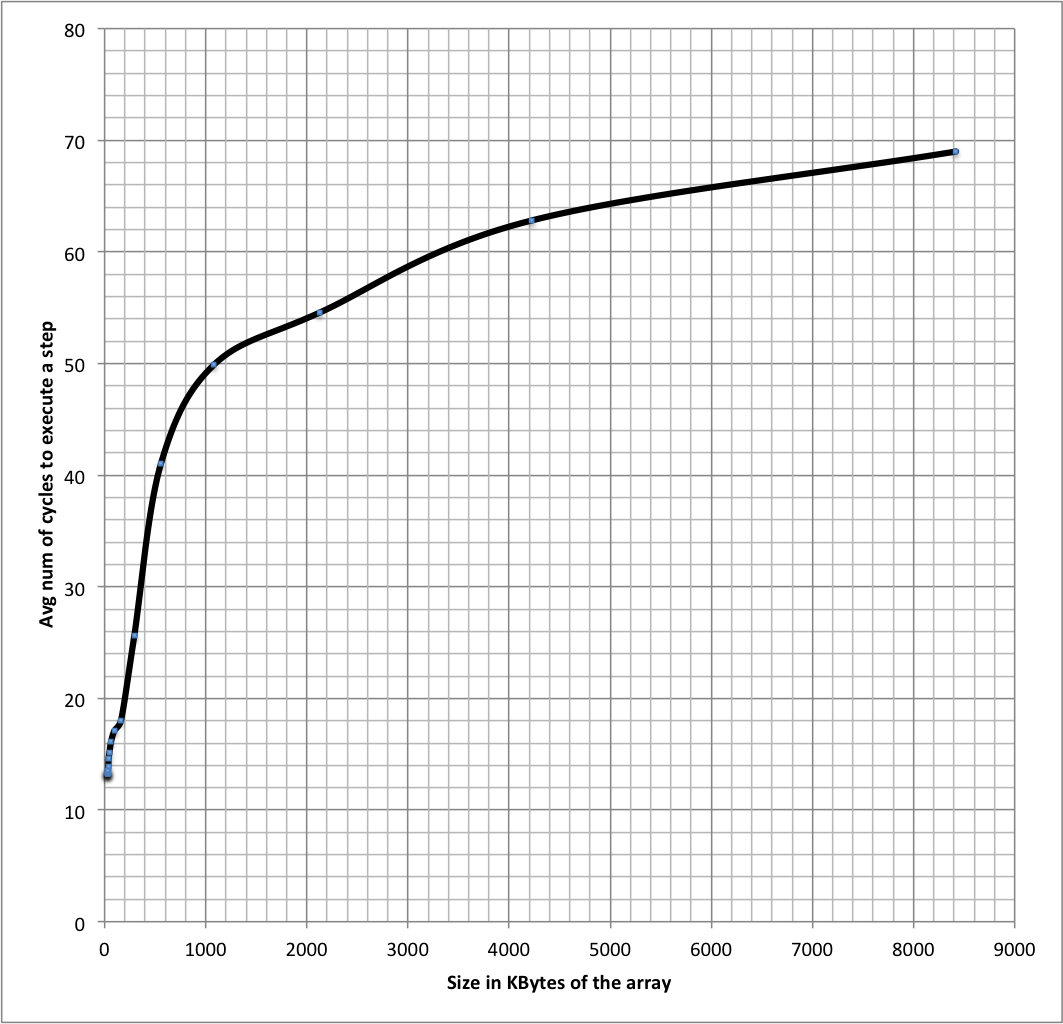
\includegraphics[width=0.8\textwidth]{graph_ptr.png}
\caption{Avg number of cycles to execute a step and the size of the array}
\label{fig:awesome_image}
\end{figure}

\noindent As the size of the array increases, so does the average number of cycles to execute a step. This is caused by the larger amount of memory accesses that the program needs to perform with increasing array size. The change in the slope happens when the array is about 1MByte large, because the proportion of L1 cache misses for smaller sizes is larger than the proportion of L2 cache misses for the larger sizes. \\[10pt]

\noindent\emph{How can we make sure that the steps are not being pipelined:}\\*
Pipelining would not affect our benchmark since each step is strictly dependent on the previous step. i.e. each step needs to wait for the address that the previous step is fetching to fetch the next address.
\pagebreak

\noindent\emph{BONUS:}\\*
Given an initialised int array with n ints, randPerm modifies the given array so that it contains all the ints from 0 to n-1 in random order in a way the pointer chase routine will access every value of the array. This task is achieved by creating a random \href{http://mathworld.wolfram.com/PermutationCycle.html}{cycle representation of the permutation} of $\{0, ... , n-1\}$ and by converting it into a 2 by n matrix representation, where the first row represents the origin and the second row represents the destination. This matrix representation as a 1-to-1 correspondence with a C-array representation where the first row gets mapped to addresses and the second row gets mapped to the corresponding values of those addresses. This routing ensures that the pointer chase will go through cycles of length n, because of the way a permutation cycle is defined and how we construct the respective array for the pointer chase. With a small modification we could create random permutations of a set n with any cycle recipe.


\begin{lstlisting}[label=some-code,caption=Random Permutation with 1 cycle]

/* Sets ARRAY to an array representation of an                                  
   N-Permuation with one cycle.*/
void shuffleArray1c(int array[], int size) {
  // init random cycle permutation  array of size SIZE
  int * cycle_array = (int *)malloc(size * sizeof(int));
  shuffleArray(cycle_array, size);
  
  //corner case: glue the two ends of the cycle together
  array[cycle_array[size - 1]] = cycle_array[0];

  //go through the cycle permutation array to construct the result array
  for (int i = 0; i < size - 1; i += 1) {
    array[cycle_array[i]] = cycle_array[i + 1];
  }
  free(cycle_array);
}

/* Initializes ARRAY of size SIZE to (0, ..., SIZE-1)   
   and shuffles it using Fisher-Yates algorithm. */
void shuffleArray(int array[], int size) {
  //initialize array (0, ..., size - 1)
  for (int i = 0; i < size; i += 1)
    array[i] = i;

  //seed the random number generator with the current time
  srand(time(NULL));

  //shuffle array using Fisher-Yates algorithm
  for (int i = 0; i < size; ++i) {
    int rand_index = rand() % size;
    int t = array[i];
    array[i] = array[rand_index];
    array[rand_index] = t;
  }
}
\end{lstlisting}


\section{Measuring Memory Bandwidth}

\noindent\emph{Average bandwidth vs the size of the array}\\*
The followings are plots showing the relationship between the average bandwidth (in Mbps) sustained by the memory system and the total size (in bytes) of the array for each of the three copy routines, our own routine, simd\_memcpy and simd\_memcpy\_cache. The size of the array varies  from 32 kilobytes to 8 megabytes. 

\begin{figure}[h]
\centering
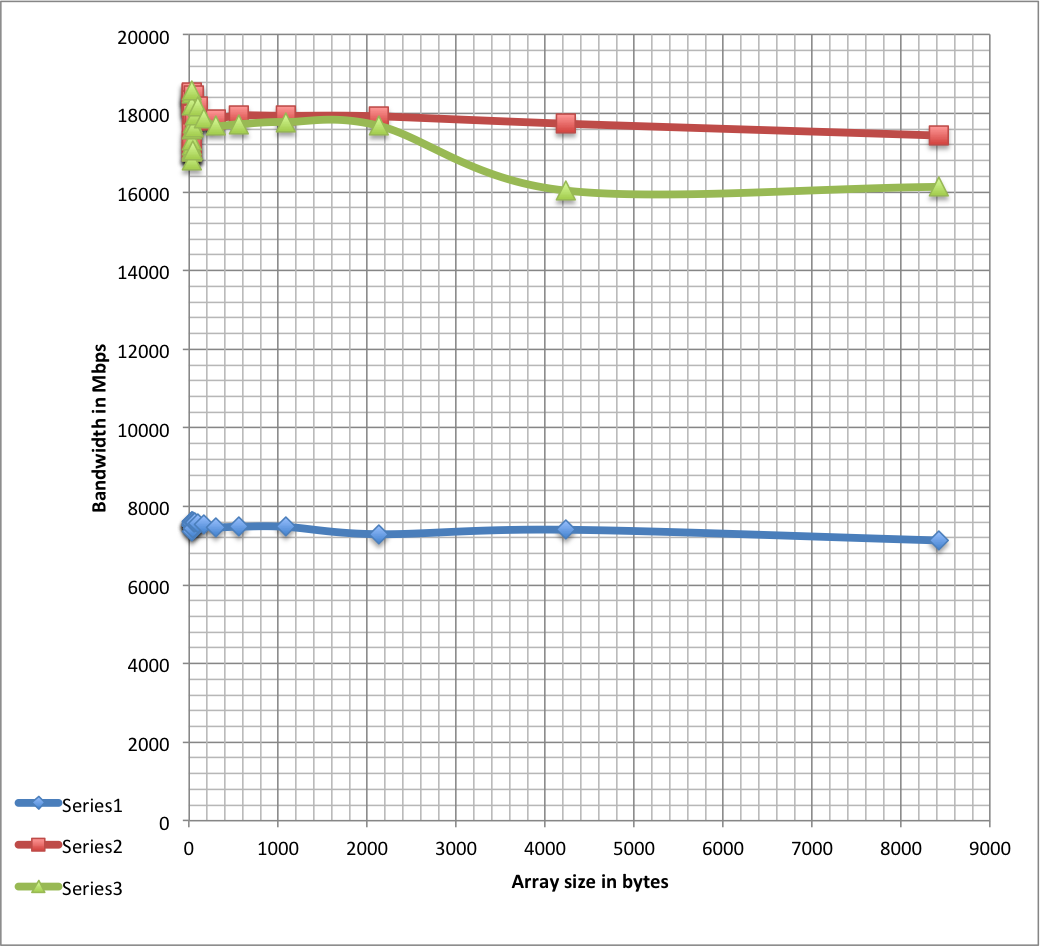
\includegraphics[width=0.8\textwidth]{graph_mem.png}
\caption{series 1: inefficient routine; series 2: simd\_memcpy; series 3: simd\_memcpy\_cache}
\label{fig:awesome_image}
\end{figure}

\noindent\emph{Discuss the shape of the curve:}\\*
The drop in memory bandwidth around 2MB is due to the fact that by copying larger arrays, we are beginning to utilise L3 cache more. Hence we reduce the average bandwidth by having to fetch data from cache with lower bandwidth more often.\\[10pt]

\noindent\emph{Why is it necessary to warm up the cache:}\\*
We are doing a performance test against a system that usually has  a high number of hits. Without the warm-up we would get false number because of the initial compulsory misses.\\[10pt]

\noindent\emph{Why an inefficient  copying procedure would yield an inaccurate measure of the maximum bandwidth:}\\*
Because it will utilise lower level caches or memories more frequently than it could achieve by optimising the code. Lower level caches and memories have less bandwidth and hence by having to access them more frequently the average bandwidth gets lower than the maxim possible average bandwidth.


\noindent\emph{Explain the SSE instructions:}\\*
\begin{itemize}
\item \textsf{\_mm\_prefetch (char const* p, int i)}: Fetch the line of data from memory that contains address p to a location in the cache hierarchy specified by the locality hint i.
\item \textsf{\_mm\_load\_si128 (\_\_m128i const* mem\_addr)}: Load 128-bits of integer data from memory into dst. mem\_addr must be aligned on a 16-byte boundary or a general-protection exception will be generated.
\item \textsf{\_mm\_stream\_si128 (\_\_m128i* mem\_addr, \_\_m128i a)}: Store 128-bits of integer data from a into memory using a non-temporal memory hint. mem\_addr must be aligned on a 16-byte boundary or a general-protection exception will be generated.
\item \textsf{\_mm\_store\_si128 (\_\_m128i* mem\_addr, \_\_m128i a)}: Store 128-bits of integer data from a into memory. mem\_addr must be aligned on a 16-byte boundary or a general-protection exception will be generated.
\end{itemize}




\section{Measuring Flops and IPC}

\begin{center}
  \begin{tabular}{ l | c | r }

       & IPC & GFlops \\ \hline
    simd & 2.34 & 9.175 \\ \hline
    scalar1 & 2.60 & 1.104 \\ \hline
    scalar0 & 0.73 & 0.874 \\ \hline
    naive & 0.33 & 0.195 \\

  \end{tabular}
\end{center}

\noindent\emph{Floating point operations performed to multiply square matrices of size n:}\\*
We require $n$ multiplications and $n - 1$ summations to perform the dot product of two vectors of size $n$. An there are $n^2$ such dot products we need to perform. Hence, the number of floating point operations ($F$) to multiply square matrices of size n is: 
$$F = (2n - 1) \cdot n^2$$\\[10pt]

\noindent\emph{How can you have $IPC > 1$:}\\*
Say the we have a simple architecture that has an $IPC = 1$. If we can combine this architecture with another equal architecture in some smart way we could have $IPC = 2$. Processors that implement superscalar architecture could achieve $IPC > 1$. \\[10pt]

\noindent\emph{Why a higher IPC is not always an indicator of an efficient program:}\\*
Because we could write a program that could achieve the same task by utilising half the the instructions that is utilising right now. The second IPC would lower than the first one, but the time it takes to execute second program could be worse than the first one. 

\end{document}








% \begin{lstlisting}[label=some-code,caption=Some Code]
% public void here() {
% 	goes().the().code()
% }
% \end{lstlisting}








